\section{MOS Stromspiegel}

\begin{minipage}[t]{0.48\columnwidth}
    Stromspiegel werden in \textbf{jeder} analogen integrierten Schaltung eingesetzt.
    Die möglichen Anwendungen sind:
\end{minipage}
\hfill
\begin{minipage}[t]{0.48\columnwidth}
    \begin{itemize}
        \item um Arbeitspunkte einzustellen
        \item als Eingangsstufen von OpAmps
        \item als grosse Lastwiderstände in Verstärkerschaltungen
    \end{itemize}
\end{minipage}


\subsection{Widlar Stromspiegel (Einfache Stromspiegel)}

\begin{minipage}[c]{0.35\columnwidth}
    \raggedright
    \begin{outline}
        \1 Drei Anschlüsse: \\
            SUPPLY, IN, OUT
        \1 Eingangstransistor als \textbf{Diode} beschaltet
        \1 \textbf{Ausgangstransistor muss in Sättigung bleiben}
        \1 $V_{\rm GS,1} = V_{\rm GS,2}$
    \end{outline}
\end{minipage}
\hfill
\begin{minipage}[c]{0.64\columnwidth}
    % \begin{tabular}{c c@{}}
    %     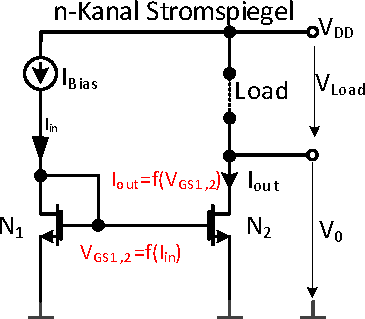
\includegraphics[height=2.3cm]{images/06_stormspiegel_nKanal.pdf} & 
    %     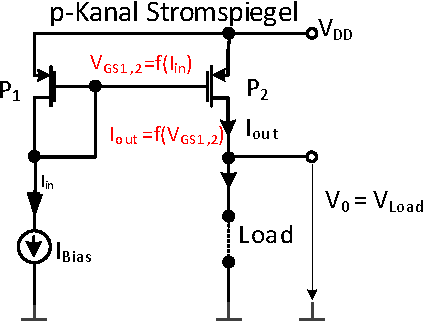
\includegraphics[height=2.3cm]{images/06_stormspiegel_pKanal.pdf}
    % \end{tabular}

     \begin{tabular}{c c@{}}
        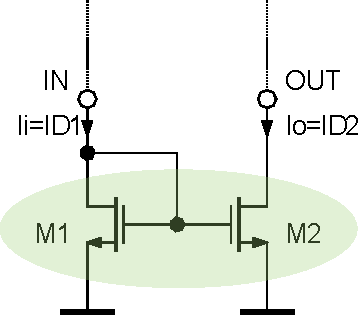
\includegraphics[height=2.2cm]{images/06_stormspiegel_widlar_nKanal.pdf} & 
        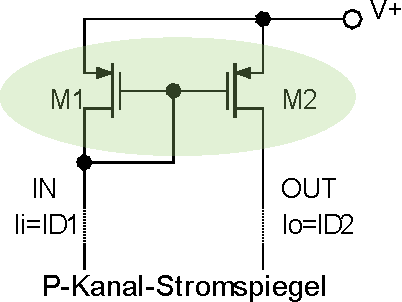
\includegraphics[height=2.2cm]{images/06_stormspiegel_widlar_pKanal.pdf}
    \end{tabular}
    
\end{minipage}


\paragraph{Wichtige Parameter}  % CHECK [Simi]: Ich weiss nicht so recht wo hin mit diesem Zeug...

\begin{minipage}[t]{0.48\columnwidth}
    \begin{outline}
        \1 Ausgangsstom $I_\text{out}$ berechnet sich aus Stromspiegelverhältnis $k$
    \end{outline}
\end{minipage}
\hfill
\begin{minipage}[t]{0.48\columnwidth}
    \begin{outline}
        \1 Eingangsimpedanz (real): $r_i = \qty{0}{\ohm}$
        \1 Ausgangsimpedanz (real): $r_o = \infty \, \qty{}{\ohm}$
    \end{outline}
\end{minipage}



\subsubsection{Arbeitspunkt festlegen}

\paragraph{Eingangsseite}

Referenzstrom aus Stromquelle oder Einstellung über Widerstand $R$

\vspace{-0.2cm}

\[
    I_\text{in} = I_\text{ref} \qquad \text{oder} \qquad I_\text{in} = \frac{V_{DD} - V_{\rm in}}{R}
\]

wobei sich die Eingangsspannung $V_{\rm in} = V_{\rm GS,1}$ aus dem Eingangsstrom berechnet als

\vspace{-0.2cm}

\[
    V_\text{in} = V_{\rm GS,1} = V_{\text{T, N}_1} + \sqrt{\frac{2 I_\text{in}}{\mu C_\text{ox}\frac{W_{\rm in}}{L_{\rm in}}}}
\]



\paragraph{Ausgangsseite}

Für Eingangs- und Ausgangstransistor soll unbedingt \textbf{das gleiche $\bm{L}$} verwendet werden.
Bei verschiedenen $L$ muss die \cbl{Kanallängenmodulation} berücksichtigt werden!

\vspace{-0.2cm}

\[
    k = \frac{I_\text{out}}{I_\text{in}} = \frac{W_\text{out}/L_\text{out}}{W_\text{in}/L_\text{in}} \cbl{ \cdot \frac{1 + \lambda_{\rm out} \cdot V_{\rm DS,out}}{1 + \lambda_{\rm in} \cdot V_{\rm DS,in}} }   \qquad \quad
    V_\text{out} \geq V_\text{DS, sat $\text{N}_2$} = \sqrt{\frac{2 I_\text{out}}{\mu C_\text{ox}\frac{W_{\rm out}}{L_{\rm out}}}}
\]

\subsubsection{Kleinsignalersatzschaltung / Kleinsignalparameter}

\begin{minipage}[t]{0.48\columnwidth}
    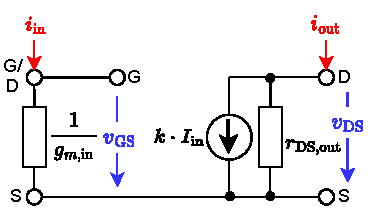
\includegraphics[width=\columnwidth, align=t]{images/06_stromspiegel_kleinsignalersatzschaltung.pdf}
\end{minipage}
\hfill
\begin{minipage}[t]{0.48\columnwidth}

    \begin{align*}
        r_{\rm in}  &\approx \frac{1}{g_{\rm m, in}} = \frac{1}{\sqrt{2 \mu C_{ox} \frac{W_{\rm in}}{L_{\rm in}} I_{\rm in}}} \\
        r_{\rm out} &= \frac{1}{g_{o1}} \approx \frac{V_{E2}}{I_{\rm out}} = \frac{a_E \cdot L}{I_{\rm out}}
    \end{align*}
    

\end{minipage}


\subsubsection{Optimierungen für kleinstmögliche Toleranzen}

\begin{tabular}{cl}
    $V_{\rm T1} = V_{\rm T2}$               & \textrightarrow\ Beide Transistoren brauchen dieselbe konstante Temperatur    \\
    $\mu C_\text{ox1} = \mu C_\text{ox2}$   & \textrightarrow\ Matching durch gute Platzierung (Common Centroid Layout)     \\
    $\lambda_1 = \lambda_2$                 & \textrightarrow\ Identische Länge $L$ (und möglichst gross) 
\end{tabular}

\smallskip

Grundsätzlich können Stromspiegel auch in Weak- und Moderate-Inversion betrieben werden.
Dabei leidet jedoch die Genauigkeit.


\subsection{Anwendungen von Stromspiegeln}

\begin{outline}
    \1 Senken-Quellen-Inversion
    \1 Verbesserung Power Supply Rejection; DC-Level Shifting \\
        \textrightarrow\ Umlenkung von $R_L$ nach GND statt Laststrom von $V_{\rm DD}$ zu Last   % NOTE: [Simi] Bild würde ich aktuell weglassen
    \1 Stromquellenlast bei Differenzstufe (siehe Abschnitt XXX) %TODO [Simi]: Referenz auf OpAmp Abschnitt, sobald existent
    \1 Erzielen eines hohen Lastwiderstands
\end{outline}


% Da $V_\text{T}$ Temperaturabhängig ist, sollten die Transistoren jeweils dieselbe Temperatur haben.

% Ebenfalls ist das Teilverhältnis von $\mu C_\text{ox}$ abhängig.
% Durch kontrolliertes Platzieren der Transistoren (Common Centroid Layout) und gute Temperaturkontrolle beim Herstellen können diese Werte relativ genau gehalten werden.

% Zu guter Letzt sollten die $\lambda$ gleich gross sein.
% Dazu müssen die Transistoren dieselbe Länge $L$ (und in einem nächsten Schritt möglichst gross) sein.


\subsection{Mehrfachstromspiegel}

%NOTE: [Simi] Wenn mehr Platz benötigt wird, Bild weglassen und nur Text verwenden

\begin{minipage}[t]{0.48\columnwidth}
    Mit einem Referenzstrom werden mehrere Ausgangsströme generiert. 
    Die Grösse der vom Stromspiegel erzeugten Ströme kann durch die Länge und Breite der Transistoren eingestellt werden.
\end{minipage}
\hfill
\begin{minipage}[t]{0.48\columnwidth}
    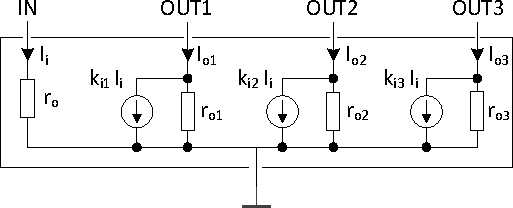
\includegraphics[width=\columnwidth, align=t]{images/06_mehrfachstromspiegel.pdf}
\end{minipage}



\subsection{Wilson-Stromspiegel (3-Transistor-Schaltung)}
Im Vergleich zum Widlar-Stromspiegel besitzt der Wilson-Stromspiegel eine \textbf{grössere Ausgangsimpedanz}.
$\text{N}_3$ bildet dabei eine Rückkopplung zur Regelung von $I_\text{o}$ auf $I_\text{i}$.
% TODO: [Flurin] How does this work? idgi...

\begin{minipage}[c]{0.35\columnwidth}
    \raggedright
    \begin{outline}
        \1 Eingangstransistor als Stromquelle beschaltet
        \1 Ausgangstransistor als \textbf{Diode} beschaltet
        \1 \textbf{T3 muss in Sättigung bleiben}
        \1 Bei gleicher Geometrie: $V_{\rm GS,2} = V_{\rm GS,3}$
    \end{outline}
\end{minipage}
\hfill
\begin{minipage}[c]{0.64\columnwidth}
     \begin{tabular}{c c@{}}
        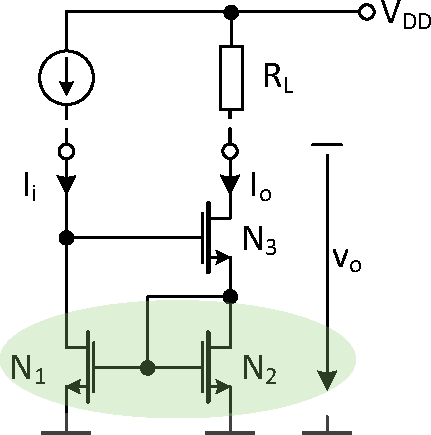
\includegraphics[height=2.9cm, align=t]{images/06_stormspiegel_wilson_nKanal.pdf} & 
        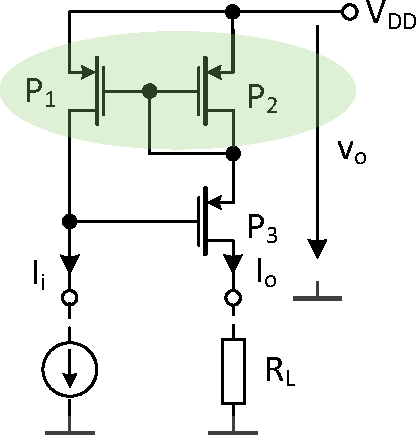
\includegraphics[height=2.9cm, align=t]{images/06_stormspiegel_wilson_pKanal.pdf}
    \end{tabular}
    
\end{minipage}


\subsubsection{Kenngrössen}
\label{Kenngrössen Wilson}

\vspace{-0.4cm}

\begin{align*}
    V_0         &\geq V_{\rm GS,2} + V_{\rm DS,sat3} = 2 V_{\rm GS} - V_T = V_T + 2 \sqrt{ \frac{2 I_O}{\mu C_{\rm OX} \frac{W_{\rm out}}{L_{\rm out}}} }                                                                                           \\
    V_I         &= 2 V_{\rm GS} = 2 V_T + 2 \sqrt{ \frac{2 I_I}{\mu C_{\rm OX} \frac{W_{\rm in}}{L_{\rm in}}} }                                                                                                                                     \\
    r_{\rm out} &\approx \frac{1}{g_{o3}} \left( 1 + \frac{g_{m3}}{g_{m2}} + \frac{1}{g_{o1}} \cdot \frac{g_{m3} g_{m1}}{g_{m2}} \right) \underset{\rm N1 = N2}{=} \frac{1}{g_o} \left( 2 + \frac{g_m}{g_o} \right) = r_{\rm DS} \cdot (2 + g_m \cdot r_{\rm DS})
\end{align*}



\subsection{Verbesserter Wilson-Stromspiegel / Kaskoden-Stromspiegel}

\begin{minipage}[t]{0.35\columnwidth}
    \begin{center}
        \textbf{\myul{Verbesserter Wilson}}

        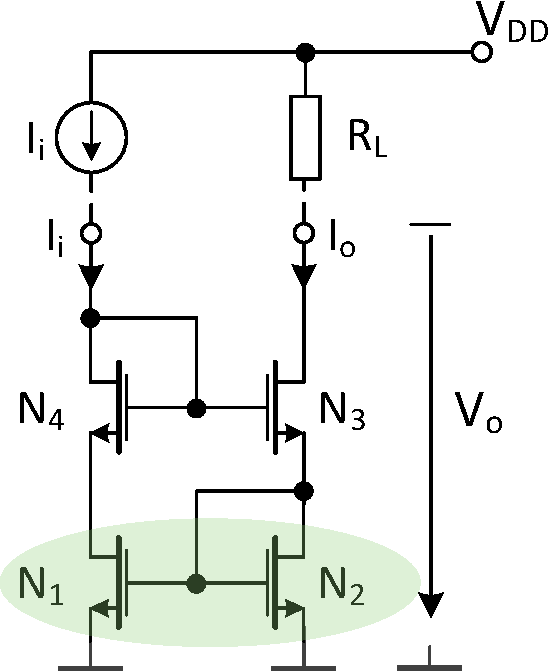
\includegraphics[width=\columnwidth, align=t]{images/06_stormspiegel_wilson_verbessert.pdf}
    \end{center}
\end{minipage}
\hfill
\begin{minipage}[t]{0.35\columnwidth}
    \begin{center}
        \textbf{\myul{Kaskode}}

        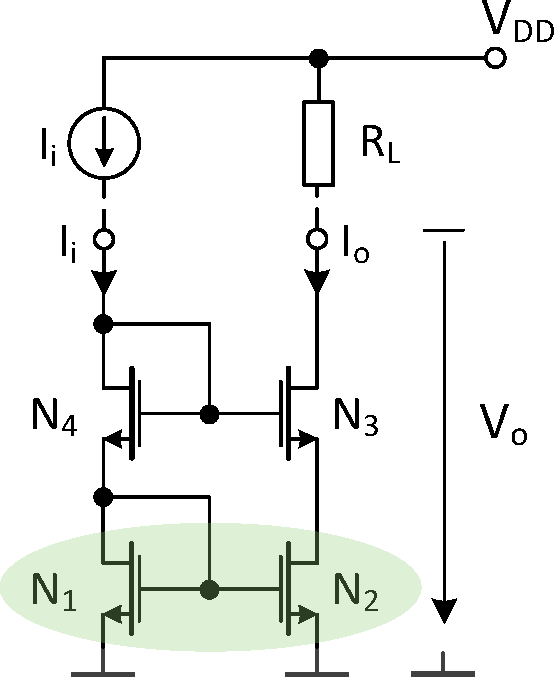
\includegraphics[width=\columnwidth, align=t]{images/06_stormspiegel_kaskode.pdf}
    \end{center}
\end{minipage}


\subsubsection{Kenngrössen}

Die Kenngrössen für beide Stromspiegel berechnen sich gleich wie diejenigen des Wilson-Stromspigels.
\textrightarrow\ Siehe Abschnitt \ref{Kenngrössen Wilson}

\columnbreak


\subsection{Stromspiegel mit geregelter Kaskode}

Durch M4 und M5 wird die Spannung am Gate von M2 konstant gehalten. % CHECK[Simi] @Flurin: Stimmt das? Auf V7 S24 steht V_{DS2} wird konstant gehalten
So wird die Ausgangsimpedanz bedeutend erhöht.


\begin{minipage}[t]{0.42\columnwidth}
    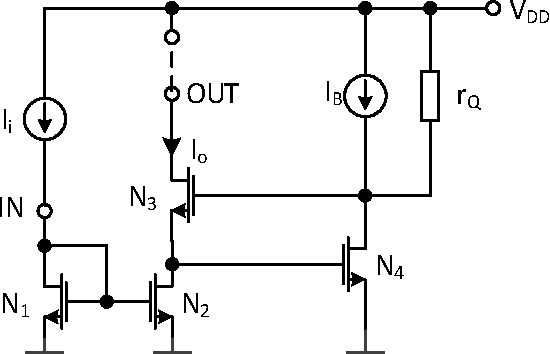
\includegraphics[width=\columnwidth, align=t]{images/06_stormspiegel_geregelte_kaskode.pdf}

\end{minipage}
\hfill
\begin{minipage}[t]{0.56\columnwidth}
    % \subsubsection{Kenngrössen}

    \vspace{-0.4cm}

    \begin{align*}
        V_0         &\geq V_{\rm GS,4} + V_{\rm DS,sat3} = V_T + (1..2) \sqrt{ \frac{2 I_O}{\mu C_{\rm OX} \frac{W_{\rm out}}{L_{\rm out}}} }                                                                                           \\
        V_I         &= V_{\rm GS,1} = 2 V_{T,1} + \sqrt{ \frac{2 I_{\rm in}}{\mu C_{\rm OX} \frac{W_{\rm in}}{L_{\rm in}}} }                                                                                                                                     \\
        r_{\rm out} &\approx \frac{1}{g_o} \left( \frac{g_m}{g_o} \right)^2 = r_{\rm DS} \cdot (g_m r_{\rm DS})^2
    \end{align*}
\end{minipage}


\subsection{Gegenüberstellung der Stromspiegel}

%NOTE [Simi] Sooo viel bringt diese Tabelle auch nicht... Die ganze Info steht bei der jeweiligen Schaltung aber bei genug Platz kann man sie schon drin lassen -> Inhalt ist aber eher klein...
\resizebox{\columnwidth}{!}{
    \renewcommand{\arraystretch}{2}
    \begin{tabular}{|c|c|c|c|c|}
    \hline
    \textbf{Typ}    & \textbf{Genauigkeit}  & $\bm{r_{\rm out}}$                                            & $\bm{V_{\rm I}}$                                                              & $\bm{V_{\rm O,min}}$                                                              \\
    \hline
    Widlar          & +                     & $\frac{1}{g_o}$                                               & $\approx V_T + \sqrt{ \frac{2I_I}{\mu C_{\text{ox}} \frac{W_I}{L_I}} }$       & $\approx \sqrt{ \frac{2I_O}{\mu C_{\text{ox}} \frac{W_O}{L_O}} }$                 \\
    \hline
    Wilson          & +                     & $\approx \frac{1}{g_o} \left( 2 + \frac{g_m}{g_o} \right)$    & $\approx 2V_T + 2 \sqrt{ \frac{2I_I}{\mu C_{\text{ox}} \frac{W_I}{L_I}} }$    & $\approx V_T + 2 \sqrt{ \frac{2I_O}{\mu C_{\text{ox}} \frac{W_O}{L_O}} }$         \\
    \hline
    Verb. Wilson    & ++                    & $\approx \frac{1}{g_o} \left( 2 + \frac{g_m}{g_o} \right)$    & $\approx 2V_T + 2 \sqrt{ \frac{2I_I}{\mu C_{\text{ox}} \frac{W_I}{L_I}} }$    & $\approx V_T + 2 \sqrt{ \frac{2I_O}{\mu C_{\text{ox}} \frac{W_O}{L_O}} }$         \\
    \hline
    Kaskode         & ++                    & $\approx \frac{1}{g_o} \left( 2 + \frac{g_m}{g_o} \right)$    & $\approx 2V_T + 2 \sqrt{ \frac{2I_I}{\mu C_{\text{ox}} \frac{W_I}{L_I}} }$    & $\approx V_T + 2 \sqrt{ \frac{2I_O}{\mu C_{\text{ox}} \frac{W_O}{L_O}} }$         \\
    \hline
    Ger. Kaskode    & ++                    & $\approx \frac{1}{g_o} \left( \frac{g_m}{g_o} \right)^2$      & $\approx V_T + \sqrt{ \frac{2I_I}{\mu C_{\text{ox}} \frac{W_I}{L_I}} }$       & $\approx V_T + (1..2) \sqrt{ \frac{2I_O}{\mu C_{\text{ox}} \frac{W_O}{L_O}} }$    \\
    \hline
    \end{tabular}
    \renewcommand{\arraystretch}{1}
}

%TODO: [Flurin] Plots der verschidenen Varianten V7S24
% Evtl. bessere Darstellungen? Warscheindlich nicht lohnenswert.
% NOTE: [Simi] Würde ich komplett wegglassen

